\subsection{Comparison with general circulation model predictions}

General circulation models are very powerful tools to understand the climate of planetary atmospheres and the
interplay between different processes at planetary scales. In the case of Titan, circulation and haze are linked
by a strong feedback loop. The large-scale structures in the haze layer are produced by the action of the
circulation. The haze layer produces a feedback effect on the circulation through the control of the stratospheric
thermal structure \citep{Rannou2004}. The detached haze is one of the noticeable features produced by the the
stratospheric circulation \citep{Rannou2002, Lebonnois2012, Larson2015}. Figures.~\ref{fig:gcm_winter}
and \ref{fig:gcm_spring} show the maps of haze extinction obtained by \cite{Lebonnois2012} and
\cite{Larson2015} at 700 nm and 525 nm respectively. They can be compared with the extinction map derived
with ISS in the CL1-UV3 filters at 338 nm.

\begin{figure}[!ht]
    \centering
    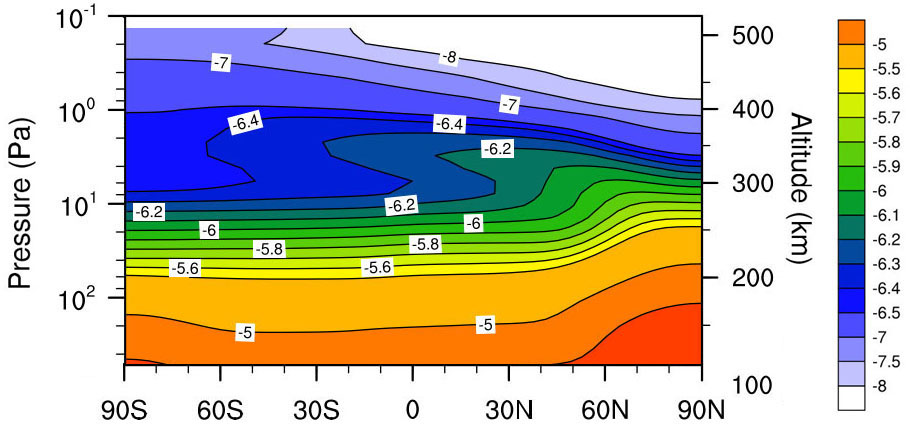
\includegraphics[width=.4\textwidth]{Fig/Lebonnois2012_Fig4_winter.jpg}
    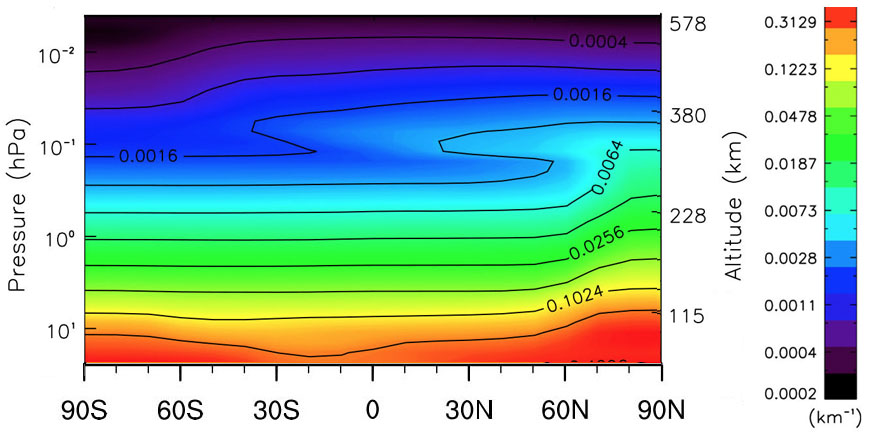
\includegraphics[width=.4\textwidth]{Fig/Larson2015-Fig7_Winter.jpg}
    \includegraphics[width=.8\textwidth]{Fig/N1477222048_2-lat_beta.png}
    \caption{At the top, the zonally-averaged haze extinction at northern winter solstice
        ($L_s = \ang{270}$) estimated by \cite{Lebonnois2012} at the wavelength $\lambda = $ 700 nm (left)
        and by \cite{Larson2015} at $\lambda = $ 525 nm (right). At the bottom, haze extinction map
        retrieved from Cassini/ISS observation CL1-UV3 ($\lambda = $ 338 nm) in the middle of winter
        (\textbf{N1477222048\_2} - $L_s = \ang{300}$).}
    \label{fig:gcm_winter}
\end{figure}

At the northern winter solstice (Fig.~\ref{fig:gcm_winter}), the detached haze appears around 350 km
in both models. In \cite{Lebonnois2012}, the altitude decreases by about few tens of km from the southern latitudes to
the north polar region where it merges with the north polar hood at \ang{40}N. In \cite{Larson2015}, the detached
haze remains at constant altitude, appears better marked than in \cite{Lebonnois2012}, and merges with the polar hood
around \ang{60}N. In both models, the extinction increases from the south to the north by about half a magnitude.
In the observations made in 2004, \emph{i.e.} at the middle of winter, the detached haze layer is completely developed at
500 km and covers latitudes from the south polar region to \ang{60}N where it merges with the north polar hood. The
location of the depletion zone decreases from 475 to 425 km between \ang{40}N and \ang{60}N, which is not the case in
models. It is, on the other hand, consistent with the results obtained from stellar occultation by \cite{Sicardy2006}.
The haze extinction increases from the south to the north with about the same magnitude as in the models. This
is consistent with a layer increasing in aerosol loading while the airmass is flowing from south to north. It was already
noted \citep{West2011, West2018} that the detached haze layer in models appears as a supplementary layer added to
the background aerosols while, in data, it appears detached because there is a zone strongly depleted in
aerosols. Finally, as mentioned earlier, the detached haze layer is continuous all around the South Pole, which is not
the case in the models.

\begin{figure}[!ht]
    \centering
    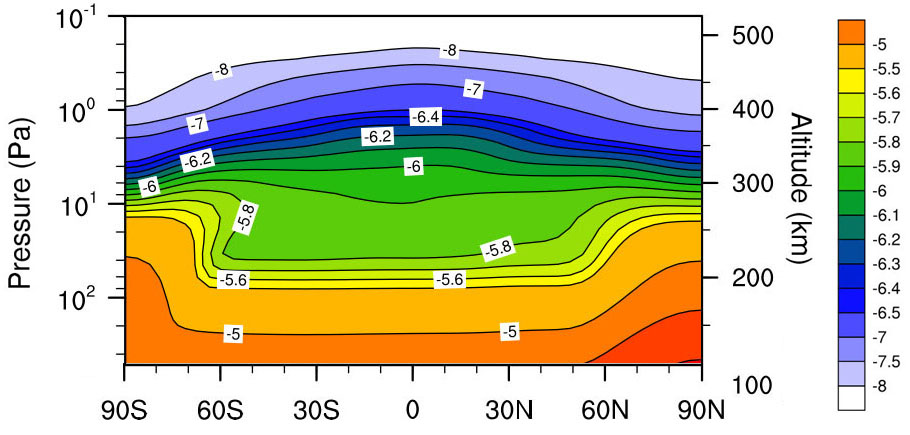
\includegraphics[width=.4\textwidth]{Fig/Lebonnois2012_Fig4_equinox.jpg}
    \includegraphics[width=.4\textwidth]{Fig/Larson2015-Fig7_Spring.jpg}
    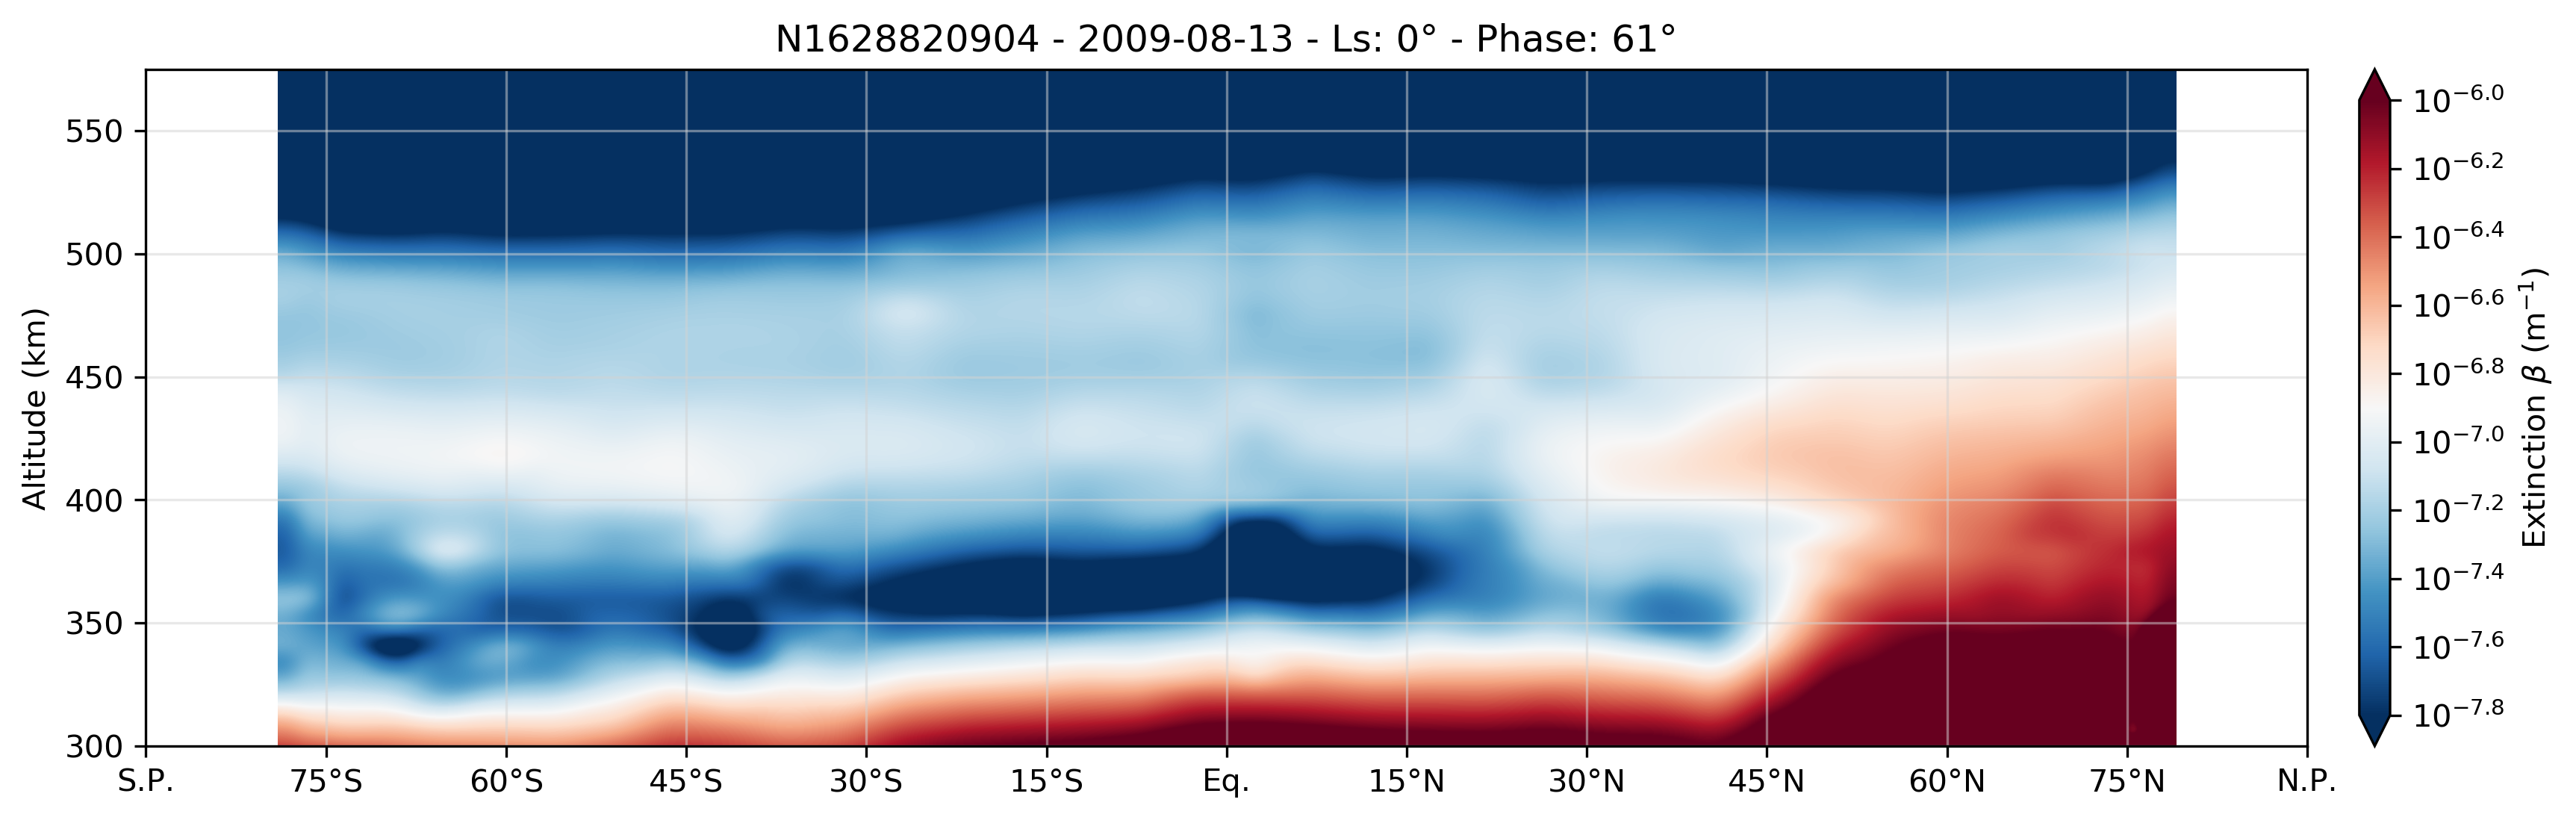
\includegraphics[width=.8\textwidth]{Fig/N1628820904_1-lat_beta.png}
    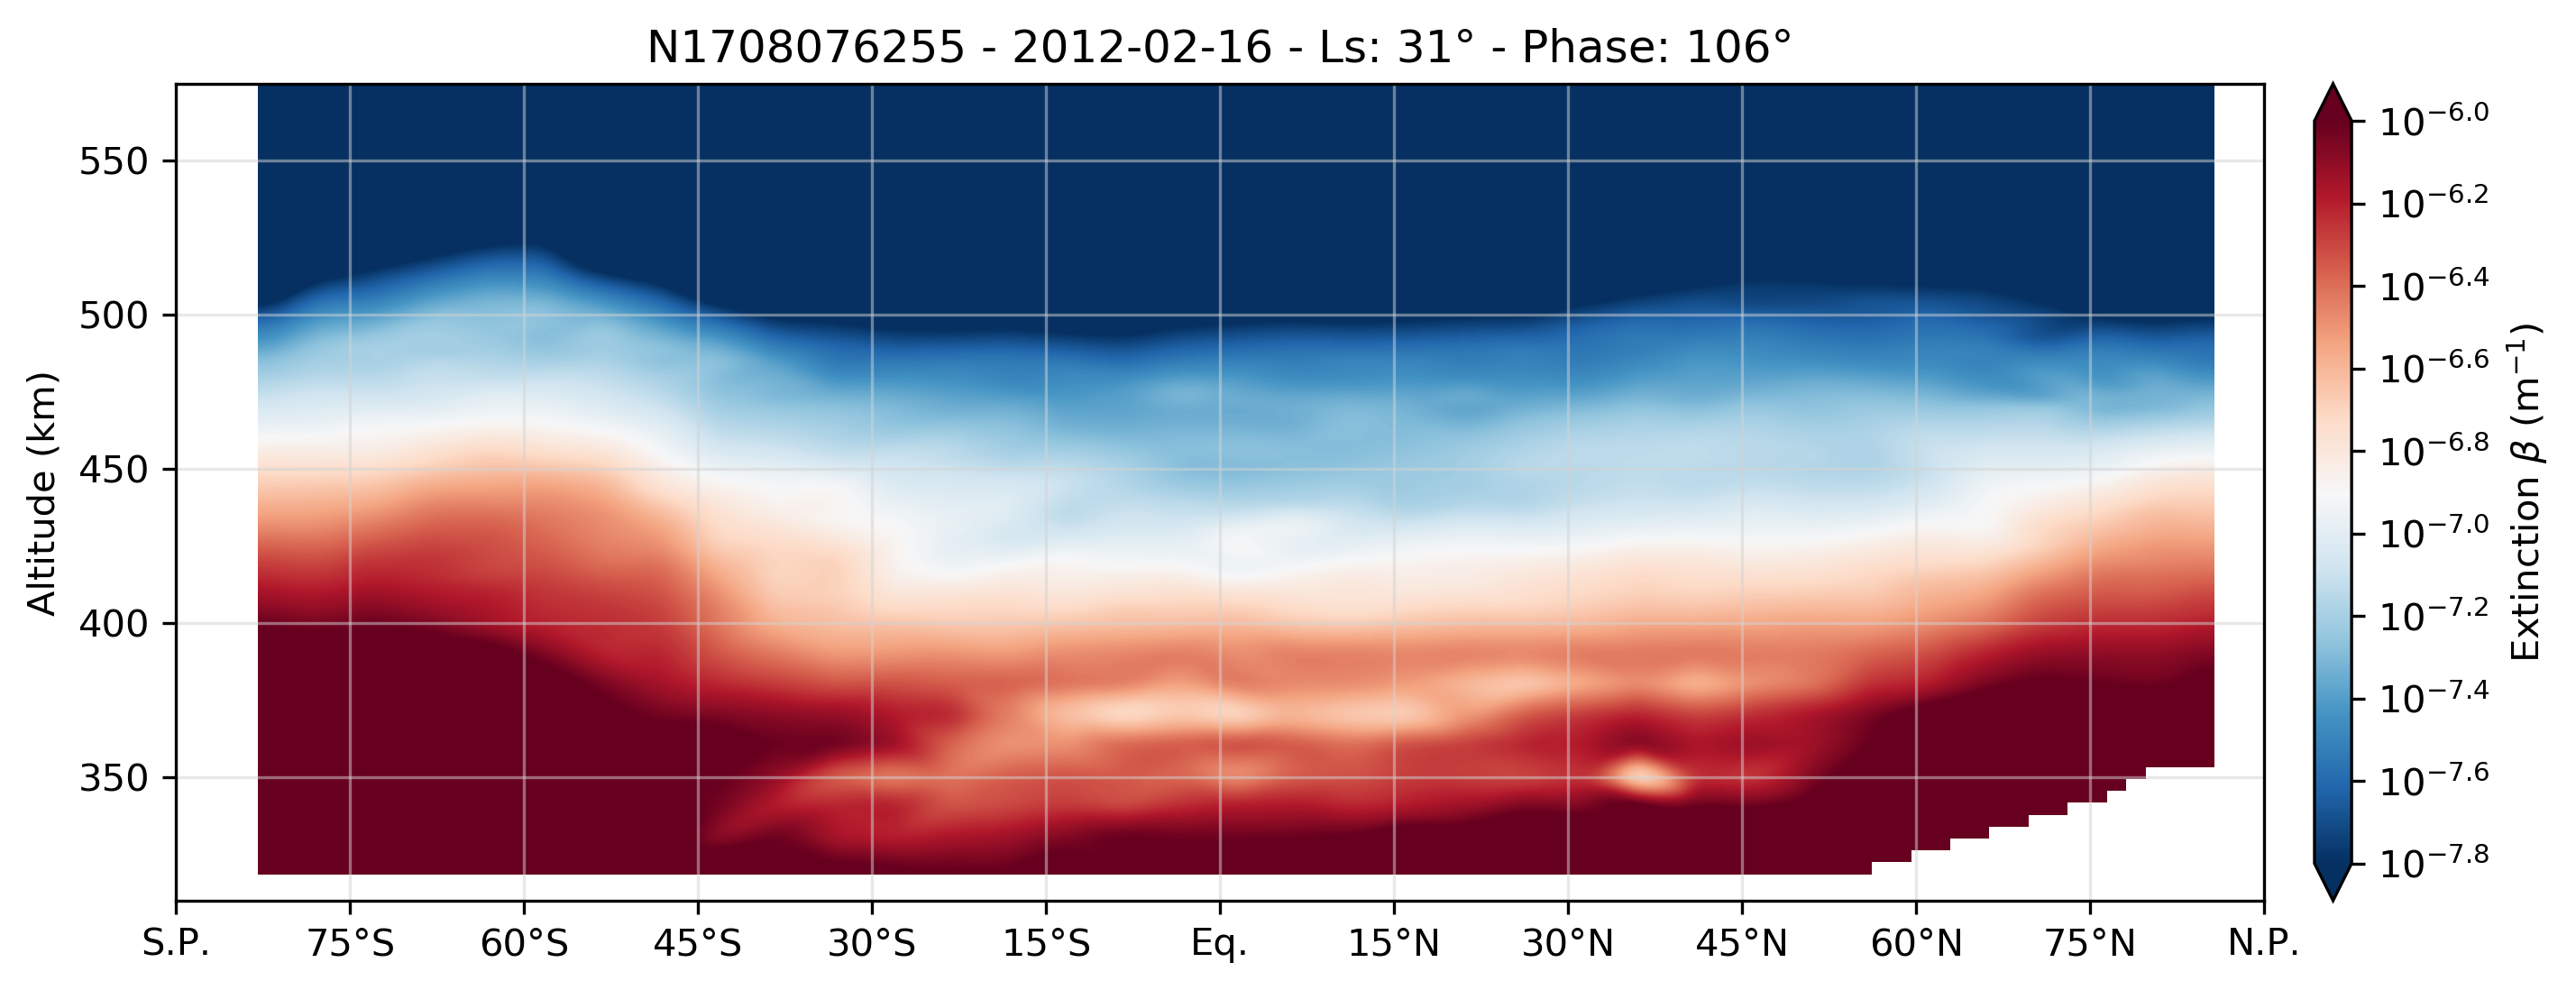
\includegraphics[width=.8\textwidth]{Fig/N1708076255_1-lat_beta.png}
    \caption{At the top, rescaled zonally averaged haze extinction at the northern spring equinox ($L_s = \ang{3}$)
        estimated by \cite{Lebonnois2012} (left) and at 1000 days after the equinox ($L_s = \ang{30}$)
        by \cite{Larson2015} (right).
        At the bottom, two panels showing the haze extinction map retrieved from the Cassini/ISS observations
        at the Northern Spring equinox (\textbf{N1628820904\_1} - $L_s = \ang{0}$) and 1000 days after the equinox
        (\textbf{N1708076255\_1} - $L_s = \ang{30}$).}
    \label{fig:gcm_spring}
\end{figure}

At the northern spring equinox (Fig.~\ref{fig:gcm_spring}), the model from \cite{Lebonnois2012} shows a
flat main haze layer without a detached haze between \ang{60}S and \ang{60}N and with two major increases at both poles. The
haze in the south is increasing as a consequence of the circulation reversal while the northern haze is diminishing
and will disappear later in the season. In observations (first panel of Fig.~\ref{fig:gcm_spring}),
this thicker haze is observed only for the northern latitudes, the detached haze has not yet disappeared
and the feeding of the south polar haze has not started. To notice a major increase of extinction at the South Pole,
we need to wait until the beginning of spring at $L_s = \ang{30}$ (second panel Fig.~\ref{fig:gcm_spring}).
At that time, the detached haze layer almost completely collapsed into the main haze and the haze distribution is very
similar to the one predicted by \cite{Lebonnois2012} at the equinox. In \cite{Larson2015}, 1000 days after the equinox,
we also observed a \emph{U} shape in the meridional haze extinction distribution as in data, but in this case, a new detached haze layer already
started to grow from the South Pole in the model, whereas in data (second panel  of Fig.~\ref{fig:gcm_spring}) the local
increase seen at 380 km is the consequence of the drop of a previous secondary layer (cf. Figs.~\ref{fig:dhl_2008_2012}g
and \ref{fig:dhl_2008_2012}h). In both comparisons, this means that the timing in the circulation models is not completely in
phase with the observations. The model of \cite{Lebonnois2012} seems to be in advance by about 3 years compared to the data.
We do not have enough information to characterize the advance in phase of \cite{Larson2015} model.

The timing and the scale of the drop predicted by both models (Fig.~\ref{fig:gcm_cycle}) globally matches
the observations after the vernal equinox. The abrupt decrease of the vertical winds could be the cause of the fall of
the detached haze layer at the aerosol terminal speed \citep{West2018}. On the other hand, the timing and the scale of the reappearance
of the detached haze layer in models does not follow exactly the observations. Anticipated in late 2014 or early 2015
($L_s = \ang{60}$) by \cite{Larson2015} or in mid-2017 ($L_s = \ang{90}$) by \cite{Lebonnois2012}, the detached haze layer
finally reappeared in late 2015 to early 2016 ($L_s = \ang{74}$).
However, in May 2017, the upper atmosphere of Titan was still evolving and did not show a polar hood in the South Pole
similar to the one observed in 2004. Moreover, the most recent observations of mid-2017 seem to show that the seasonal
formation of the detached haze layer could be different from one hemisphere to the other. The double peaks at
420 and 450 km in the temperature gradient profile, a proxy for the haze extinction, obtained from the 1989
occultation \citep{Sicardy1999} supports this hypothesis.

\begin{figure}[!ht]
    \centering
    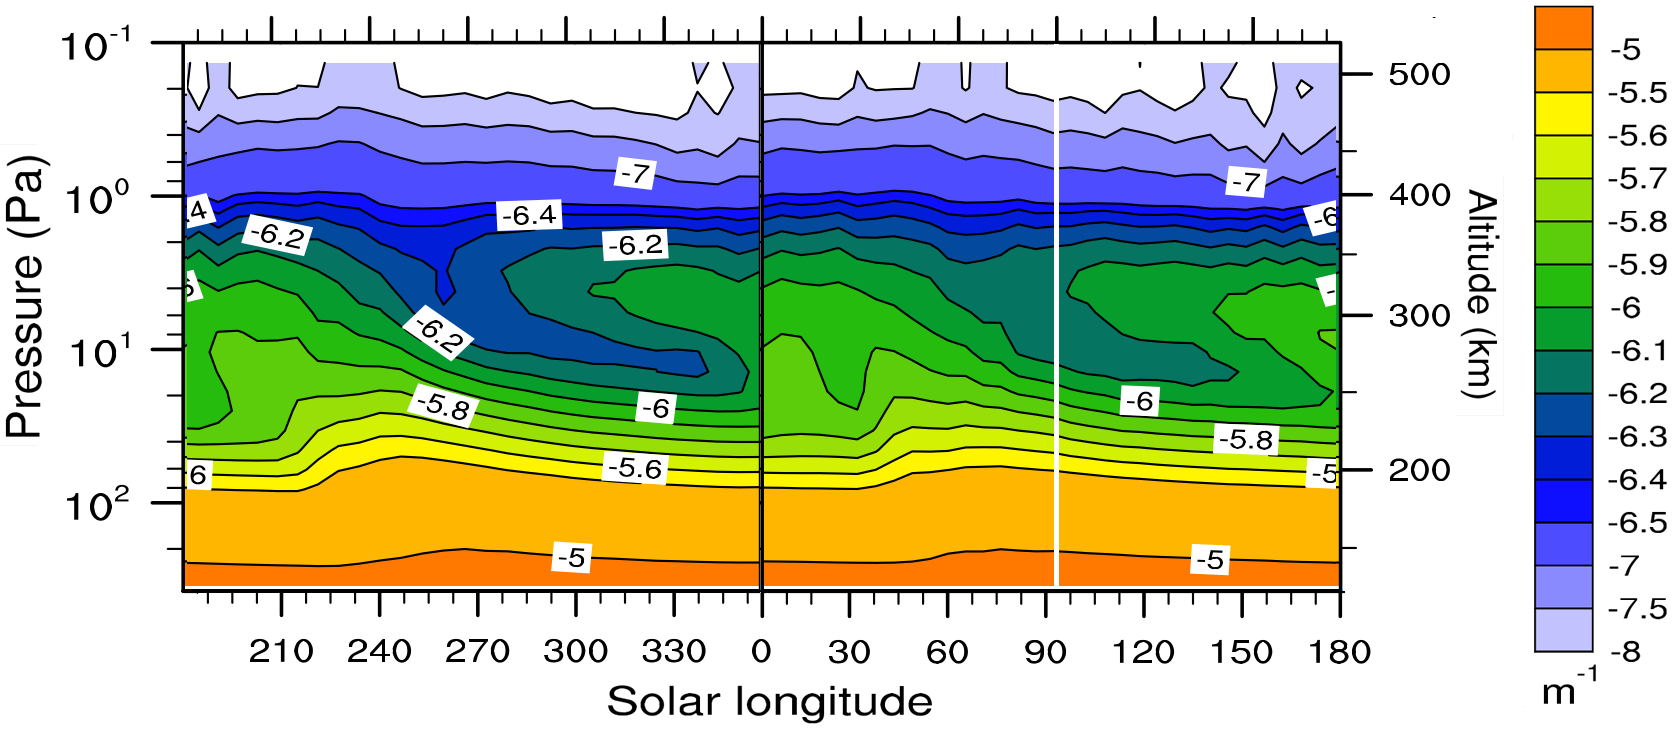
\includegraphics[width=.4\textwidth]{Fig/Lebonnois2012_dhl_cycle.png}
    \includegraphics[width=.4\textwidth]{Fig/Larson2015_dhl_cycle.png}
    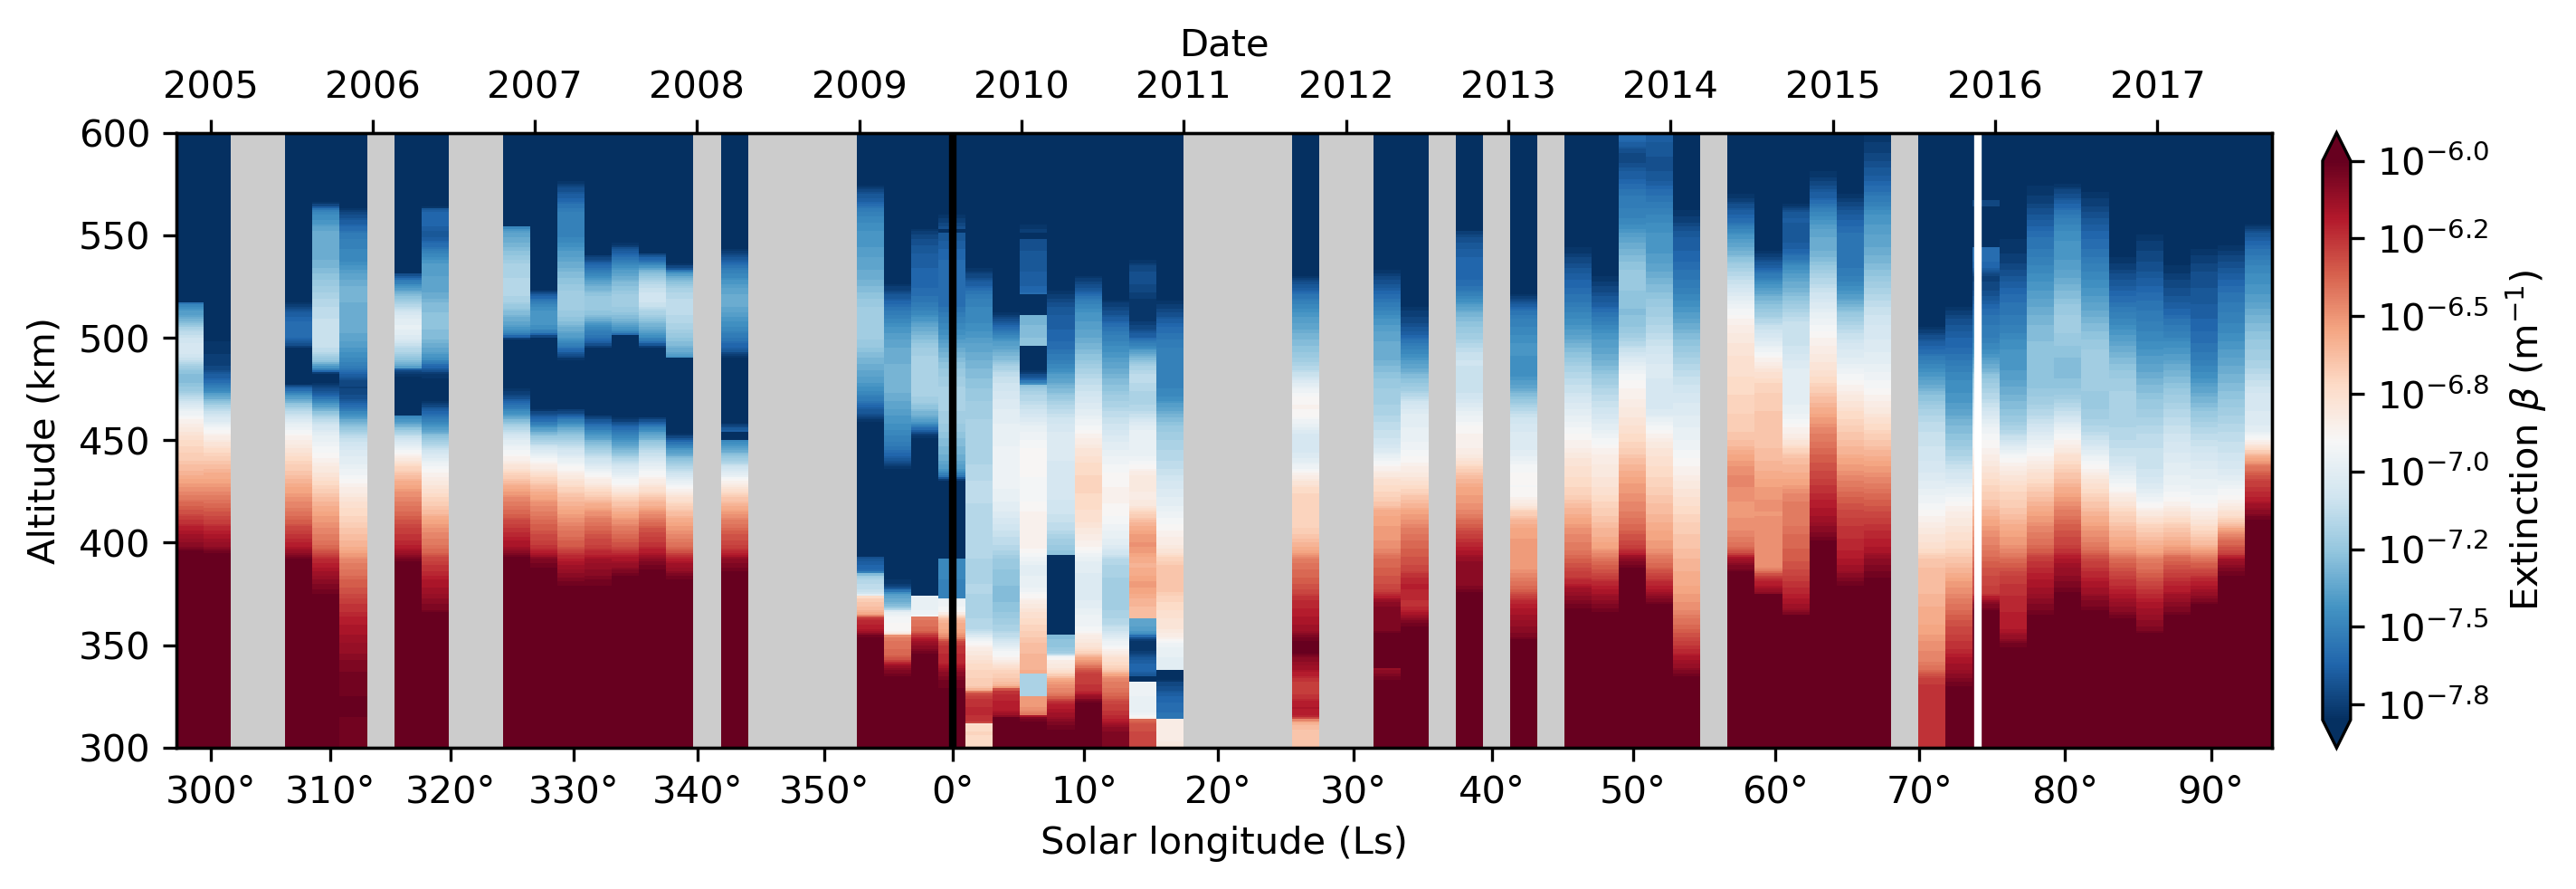
\includegraphics[width=.8\textwidth]{Fig/DHL_time_eq.png}
    \caption{Top-right: the annual variations of the zonally averaged equatorial opacity at 700 nm adapted
        from \cite{Lebonnois2012}.
        Top-left: the seasonal evolution of the aerosol mass density (g/cm$^3$) adapted from \cite{Larson2015}.
        The white dots are the local maxima of extinction extracted from the model.
        Bottom: the haze extinction as a function of time and altitude at the equator \citep[completed since][]{West2018}.
        The data are binned by 2 months ($\Delta Ls \approx \ang{2} $). The gray area corresponds to the period where
        no UV3 observations where available (see Fig.~\ref{fig:img_sampling}).
        In each figure, the black vertical line corresponds to the vernal equinox and the white vertical
        line is the date of the reappearance of the detached haze layer ($L_s = \ang{90}$, $L_s = \ang{60}$
        and $L_s = \ang{74}$ respectively).
    }
    \label{fig:gcm_cycle}
\end{figure}

The current general circulation models do not match some of the large-scale features reported earlier. The first of them
is the shape of the vertical extinction profile which has a local depletion, producing the appearance of a detached haze layer in the
observations, while in models it appears as a high altitude haze layer superimposed to the main background haze.
The amplitude of the observed depletion reported, before and during the collapse, is sufficient to consider that the
detached haze layer is really disconnected from the main haze layer. We already stressed that the detached haze layer is
continuous around the South Pole without any visible upwelling coming from the main haze at this location. Finally, we
reported an early contraction of the main haze in 2008, just before the drop of the detached haze at the equinox. The origin
for such a contraction is likely related to the weakening of the Hadley cell when the latitudinal illumination gradient
decreases around the equinox.

Thanks to high spatial resolution of the ISS NAC camera, we noticed some small-scale structures which could be unresolved or
erased by the temporal averaging in GCMs. During the northern winter and spring, we observed some sporadic decreases and
bursts in the extinction profiles at very short time scales. These events could have a major impact on the redistribution of
aerosols in the upper atmosphere. We also reported, in numerous cases, the existence of sub-layers above the main detached
haze layer with large latitude extend. Usually, their presence could be followed during more than one Earth year. This is
especially true during the collapse of the main detached haze layer after the equinox, when we observed several smaller
drops from 500 km down to 300 km. And finally, the double structure reported in 2016-2017
(Figs.~\ref{fig:dhl_2015_2017}c and \ref{fig:dhl_2015_2017}d) with two very distinct detached haze layers in the
North at 450 km, in the South at 520 km, was never mentioned before and needs a new interpretation.

We want to highlight facts that would help to better constrain the climate models. 
GCMs are ideal tools to understand the interplay of different components of Titan's climate.
But they also have several limitations which are often technical by nature (low spatial resolution, shallow water
approximation for the dynamics, radiative transfer in plane-parallel, no link with the high mesosphere and thermosphere physics).
Limitations may also come from incorrect boundary conditions. We give some remarks:

\begin{enumerate}
\item the collapse starts in the southern hemisphere and concerns the main haze and then the detached haze. This
may indicate that aerosols of the main haze and the detached haze do not have the same fractal structure. This is
already suggested by \cite{Lavvas2009} and \cite{Larson2015}.
The weakening or the displacement of ascending branch of the circulation would first affect the more
compact aerosols of the main haze before the fluffiest aerosols of the detached haze that can remain suspended more
easily.
\item the finest details found in this work occur at length scales smaller than the GCM grid scale.
ISS observations show an instantaneous snapshot of the haze layer. GCMs generally
calculate extinction of haze averaged over several Titan days and/or are zonally averaged. Comparing GCMs instantaneous and
not zonally averaged outputs would allow to see if they are able or not to produce the same kind of variabilities as
observed. These variability may also be induced by processes occurring in higher layers not modeled by the GCMs.
\item the timing offset of the DHL reappearance in GCM is probably due to the model top levels which are generally too
low. Vertical extension of the models and of the haze layer may improve the timing of the cycle.
\item the source of the aerosols depends on photochemical processes that occur far above the DHL and which are
also are subjected to circulation in the upper mesosphere and thermosphere.
Accounting for the physics and chemistry in higher layers, for instance, a coupling with thermospheric models could
be a key to understand further the detail of the haze cycle.
\end{enumerate}